% Options for packages loaded elsewhere
\PassOptionsToPackage{unicode}{hyperref}
\PassOptionsToPackage{hyphens}{url}
%
\documentclass[
  12pt,
  norsk,
]{article}
\usepackage{amsmath,amssymb}
\usepackage{lmodern}
\usepackage{ifxetex,ifluatex}
\ifnum 0\ifxetex 1\fi\ifluatex 1\fi=0 % if pdftex
  \usepackage[T1]{fontenc}
  \usepackage[utf8]{inputenc}
  \usepackage{textcomp} % provide euro and other symbols
\else % if luatex or xetex
  \usepackage{unicode-math}
  \defaultfontfeatures{Scale=MatchLowercase}
  \defaultfontfeatures[\rmfamily]{Ligatures=TeX,Scale=1}
\fi
% Use upquote if available, for straight quotes in verbatim environments
\IfFileExists{upquote.sty}{\usepackage{upquote}}{}
\IfFileExists{microtype.sty}{% use microtype if available
  \usepackage[]{microtype}
  \UseMicrotypeSet[protrusion]{basicmath} % disable protrusion for tt fonts
}{}
\makeatletter
\@ifundefined{KOMAClassName}{% if non-KOMA class
  \IfFileExists{parskip.sty}{%
    \usepackage{parskip}
  }{% else
    \setlength{\parindent}{0pt}
    \setlength{\parskip}{6pt plus 2pt minus 1pt}}
}{% if KOMA class
  \KOMAoptions{parskip=half}}
\makeatother
\usepackage{xcolor}
\IfFileExists{xurl.sty}{\usepackage{xurl}}{} % add URL line breaks if available
\IfFileExists{bookmark.sty}{\usepackage{bookmark}}{\usepackage{hyperref}}
\hypersetup{
  pdftitle={«R Notebooks» and reproducibility},
  pdfauthor={Assignment 1 i kurset Data Science 2021 - Karoline Midtbø og Morten Knutsen},
  pdflang={nb-NO},
  hidelinks,
  pdfcreator={LaTeX via pandoc}}
\urlstyle{same} % disable monospaced font for URLs
\usepackage[margin=1in]{geometry}
\usepackage{graphicx}
\makeatletter
\def\maxwidth{\ifdim\Gin@nat@width>\linewidth\linewidth\else\Gin@nat@width\fi}
\def\maxheight{\ifdim\Gin@nat@height>\textheight\textheight\else\Gin@nat@height\fi}
\makeatother
% Scale images if necessary, so that they will not overflow the page
% margins by default, and it is still possible to overwrite the defaults
% using explicit options in \includegraphics[width, height, ...]{}
\setkeys{Gin}{width=\maxwidth,height=\maxheight,keepaspectratio}
% Set default figure placement to htbp
\makeatletter
\def\fps@figure{htbp}
\makeatother
\setlength{\emergencystretch}{3em} % prevent overfull lines
\providecommand{\tightlist}{%
  \setlength{\itemsep}{0pt}\setlength{\parskip}{0pt}}
\setcounter{secnumdepth}{-\maxdimen} % remove section numbering
\ifxetex
  % Load polyglossia as late as possible: uses bidi with RTL langages (e.g. Hebrew, Arabic)
  \usepackage{polyglossia}
  \setmainlanguage[]{norsk}
\else
  \usepackage[main=norsk]{babel}
% get rid of language-specific shorthands (see #6817):
\let\LanguageShortHands\languageshorthands
\def\languageshorthands#1{}
\fi
\ifluatex
  \usepackage{selnolig}  % disable illegal ligatures
\fi
\newlength{\cslhangindent}
\setlength{\cslhangindent}{1.5em}
\newlength{\csllabelwidth}
\setlength{\csllabelwidth}{3em}
\newenvironment{CSLReferences}[2] % #1 hanging-ident, #2 entry spacing
 {% don't indent paragraphs
  \setlength{\parindent}{0pt}
  % turn on hanging indent if param 1 is 1
  \ifodd #1 \everypar{\setlength{\hangindent}{\cslhangindent}}\ignorespaces\fi
  % set entry spacing
  \ifnum #2 > 0
  \setlength{\parskip}{#2\baselineskip}
  \fi
 }%
 {}
\usepackage{calc}
\newcommand{\CSLBlock}[1]{#1\hfill\break}
\newcommand{\CSLLeftMargin}[1]{\parbox[t]{\csllabelwidth}{#1}}
\newcommand{\CSLRightInline}[1]{\parbox[t]{\linewidth - \csllabelwidth}{#1}\break}
\newcommand{\CSLIndent}[1]{\hspace{\cslhangindent}#1}

\title{«R Notebooks» and reproducibility}
\author{Assignment 1 i kurset Data Science 2021 - Karoline Midtbø og
Morten Knutsen}
\date{}

\begin{document}
\maketitle

\hypertarget{introduction}{%
\section{Introduction}\label{introduction}}

In this paper we will look at reproducibility and how R notebook can be
a solution to this problem. First we are going to look at literature
review, where we present what other scientific authors writes about
reproducing. Then we will have our on discussion on how the necessity of
reproducibility in research and whether the use of ``R - Notebooks'' is
a possible solution to the problem on lack of reproducibility. In the
end we will represent a conclusion to the chapter discussion.

When we are talking about \textbf{\emph{reproducibility}} it is about
getting confidence in the conclusion to the scientists
(\protect\hyperlink{ref-mcnutt2014}{McNutt, 2014}). The definition of
reproducibility is how other researchers can use the analysis of former
researchers to achieve the same result using the same analysis and data
(\protect\hyperlink{ref-samota2021}{Samota og Davey, 2021})

\textbf{\emph{R Notebook}} is a document from R Markdown that contains
chunks(\protect\hyperlink{ref-grolemund}{Grolemund og Wickham, u.å.}). R
Notebook is a document that has direct interaction with R, but it is
also a document that are reproducible
(\protect\hyperlink{ref-grolemund}{Grolemund og Wickham, u.å.}). When
you are going to publish the document you can publish Immediately or you
can knitted to another document like HTML,PDF or Word.

\hypertarget{short-literature-review}{%
\section{Short literature review}\label{short-literature-review}}

Roger D. Peng has written a paper that tells us more about
reproducibility. He says that ``\emph{A critical barrier to
reproducibility in many cases is that the computer code is no longer
available}'' \protect\hyperlink{ref-peng2011}{Peng}
(\protect\hyperlink{ref-peng2011}{2011}). This is one of the problems to
reproducibility. ``\emph{Researchers across a range of computational
science disciplines have been calling for reproducibility, or
reproducible research, as an attainable minimum standard for assessing
the value of scientific claims}'' \protect\hyperlink{ref-peng2011}{Peng}
(\protect\hyperlink{ref-peng2011}{2011}). Even if reproducibility
becomes a minimum standard, it does not guarantee the quality. The ``R''
kite-mark is to indicate the idea that a knowledgeable has reviewed the
data and code and found it reproducible. To make researches reproducible
it is recommended for everyone that use any computing in there research
to publish there code. Even though the code isn't clean, they should
publish it, it just need to be available
\protect\hyperlink{ref-peng2011}{Peng}
(\protect\hyperlink{ref-peng2011}{2011}).

There is on article about ``\emph{Do economics journal archives promote
replicable research?}'' written by McCullough et al.@mccullough2008. The
article show how the data and the code to an article is important to
have to replicate. There is several companies that are publishing
articles that want a system that makes the authors include the data and
code when they publish, but most of them fail to achieve that. There are
a replication policies that they can follow, that includes some
requirements, on how to do it, and then have them in archives. The
reason to many of them failed is that it is all up to the authors to do
them right. The goal of replication is that authors or researchers can
use other-minded articles to explore further, so they can avoid wasting
time doing the same research. They also talks how the economics don't
see the reason to replicate, but what else is the meaning of archives?

According to McCullough et al.~there are several authors who do not
include data and codes when they are publishing article etc. Possible
reasons why they do not publish is that they themselves have to sort to
see that all data and codes are in order, or else it is not usable to
reproduce. Sometimes they don't want to let other authors do further
research to the study they did, or to use it as a base. When it comes to
publishing with code and data, the authors have to include it by them
self in the publishing \protect\hyperlink{ref-mccullough2008}{McCullough
et al.} (\protect\hyperlink{ref-mccullough2008}{2008}).

There is some solution on how to increase the opportunities to reproduce
others work. Some articles show examples that archives can be mandatory,
that will mean the authors have to include data and code when they
publishing so the article etc. will be in a system in the archive and
can be used again later on. With help of R Markdown/R Notebook it will
be easier for the authors to have control on the code and data, and it
will always include in the program. There is to different chunks that
helps with data and coding.

Code chunks are a series of commands in different programming language,
in example R. Code chunks preform calculations needed to produce the
appropriate output. Also to create intermediate results used across
different code chunks.

A text chunk, on the other hand, describes the results, codes, problems
and the interpretation. Text chunks is formatted for the user to read
it, not the computer.

\hypertarget{discussion}{%
\section{Discussion}\label{discussion}}

R notebook can be a solution to fix the problem of reproducibility, but
only partly. R notebook has the opportunity to be a good tool for any
researcher, but it requires that the researchers knows how to use the
program and they need to have the exact same packages that was used
under the study, or else they will not manage to reproduce the study.
When you are using R studio you can use Github to store your repository,
then you can store it as private or public. After you store it in Github
you can pull it down to R studio whenever you need it. Other Github
users can also use your repository if you make it public, and use your
data and code, if they have the same packages you used. There is also a
lot researchers that want to protect their work and will not make their
codes available, and then it will be difficult to reproduce for others.
For beginners in R there will be a lot to get into, there is many
different things you need to know before you can use it, there is a lot
of programs you need to install for making it optimal.

\begin{enumerate}
\def\labelenumi{\arabic{enumi}.}
\tightlist
\item
  R Notebook will solve the problem with reproducibility
\end{enumerate}

\begin{itemize}
\tightlist
\item
  With R Notebook the document already contain codes.
\item
  It is a free program to use, everybody can install it.
\item
  You can use Github to store it longer.
\end{itemize}

\begin{enumerate}
\def\labelenumi{\arabic{enumi}.}
\setcounter{enumi}{1}
\tightlist
\item
  R notebook will not solve the problem reproducibility
\end{enumerate}

\begin{itemize}
\tightlist
\item
  If you want the data and code, you have to have the right packages
  that was used.\\
\item
  To use the program you have to know how to use it.
\end{itemize}

\texttt{\{r-første\ chunk\}\ sessionInfo()}

This function can help us to reproduce the research because it gives us
information about which R version and packages we used. It can take time
to install all the packages if you don't have them, but with chunks it
will be easier to find which packages we used in our work.

After the literature work we did, we find a lot of information about how
researchers feel about reproducibility. They want to protect the work
they did, and often they don't want to publish their code and data they
used to find their answers. Without the code and data other researchers
can't get the exact same answer, and they will have to take the same
exact test and use a lot of time to get the information. If the author
publish the code and data it will be easier for the next researcher to
just use the test that is already done and they will have the exact same
answer and can use it to develop it. When authors or researchers publish
with data and code, there will be a lot more of opportunities of
reproducibility. But it is all on the authors, when they publish they
have to check if the code and data are included.

\hypertarget{conclusion}{%
\section{Conclusion}\label{conclusion}}

After we have read different literature and had an discussion, we can
see it is a split between the authors that want to publish their data
and code and they who do not want to publish them. We conclude that the
R Notebook will help the authors or researchers to have more control on
the data and the code, but it's a program that need knowledge and
require different packages to get the exact same answer. Predictability
will help a lot when it comes to further resource, to don't waste time
on what others have answer on, it also makes it easier to back up what
they got.

\hypertarget{references}{%
\section{References}\label{references}}

\hypertarget{section}{%
\section*{\texorpdfstring{\protect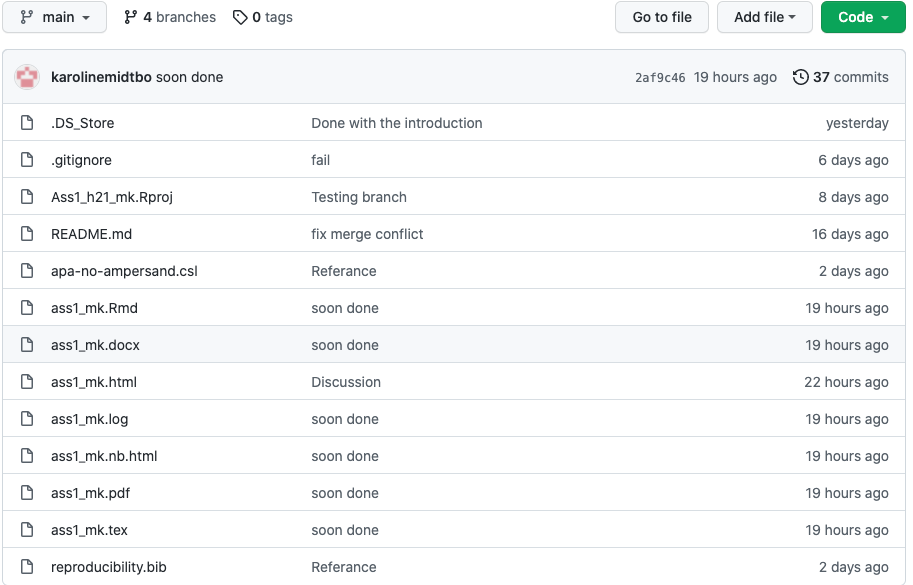
\includegraphics{images/Skjermbilde 2021-09-15 kl. 10.29.21.png}}{}}\label{section}}
\addcontentsline{toc}{section}{}

\hypertarget{refs}{}
\begin{CSLReferences}{1}{0}
\leavevmode\hypertarget{ref-grolemund}{}%
Grolemund, G., og Wickham, H. (u.å.). \emph{R for {Data Science}}.

\leavevmode\hypertarget{ref-mccullough2008}{}%
McCullough, B. D., McGeary, K. A., og Harrison, T. D. (2008). Do
Economics Journal Archives Promote Replicable Research? \emph{Canadian
Journal of Economics/Revue canadienne d'économique}, \emph{41}(4),
1406--1420. \url{https://doi.org/10.1111/j.1540-5982.2008.00509.x}

\leavevmode\hypertarget{ref-mcnutt2014}{}%
McNutt, M. (2014). Reproducibility. \emph{Science}, \emph{343}(6168),
229--229. \url{https://doi.org/10.1126/science.1250475}

\leavevmode\hypertarget{ref-peng2011}{}%
Peng, R. D. (2011). Reproducible {Research} in {Computational Science}.
\emph{Science}, \emph{334}(6060), 1226--1227.
\url{https://doi.org/10.1126/science.1213847}

\leavevmode\hypertarget{ref-samota2021}{}%
Samota, E. K., og Davey, R. P. (2021). Knowledge and Attitudes Among
Life Scientists Toward Reproducibility Within Journal Articles: A
Research Survey. \emph{Frontiers in Research Metrics and Analytics},
\emph{6}, 678554. \url{https://doi.org/10.3389/frma.2021.678554}

\end{CSLReferences}

\end{document}
